\section{Experiment 6: colour, inversion and reversal}

\subsection{Methodology}

\paragraph{Stimuli}

A 1000-frame corpus of consecutive fire images was used.



\paragraph{Subjects}

8 subjects were recruited using a mailing list operated by University College London. All reported normal or corrected-to-normal vision.

\paragraph{Trial structure}

Delayed match-to-sample with altered sample.
In each trial, a sample was presented first, followed by two tests. A manipulation was applied to the sample; the tests were unchanged. Subjects indicated which test they thought corresponded to the sample using the left arrow (first sample) and right arrow (second sample) keys. 

Sample length (sL) was one 10 frames (0.2 seconds)
Test length was 15 frames (0.3 seconds)

\paragraph{Factors}

We varied the manipulation applied to the sample clips:
none, colour-inverted, backwards, or spatially inverted.

Colour inversion was done by expressing each image in HSV space and rotating each pixel by 180 degrees about the hue axis.

\paragraph{Block structure}

Firstly, we presented 30 training trials with static samples and tests (displayed for 0.2 and 0.3 seconds respectively) with the four manipulations applied to the sample.

Next, we presented 30 training trials with dynamic samples and tests and the same clip lengths, but with samples and tests unaltered.

We used 4 block types (corresponding to each manipulation) with 4 repetitions of each block (16 blocks total) in random order.


\begin{figure}[H]
\centering
\renewcommand{\arraystretch}{1.8}

      \begin{subfigure}[b]{\textwidth}
\begin{tabular}{ >{\bfseries}r | p{8cm}   }
& \textbf{Experiment 3}\\
\hline
  
Design & 2AFC delayed match-to-sample, with filtered or inverted sample\\                   
Stimuli & 1000-frame corpus\newline
		1 second sample (50 frames)\newline
		1.2 second test (60 frames)\\
Factors & Manipulation:\newline
		a) none\newline
		b) colour inversion\newline
		c) temporal inversion\newline
		d) spatial inversion\\

Block design & Manipulation varied across blocks\newline
		4 block types \newline
		16 blocks in random order \\
Training &60 training trials \\
Subjects&8\\
\end{tabular}
\caption{Design summary.}
   \end{subfigure}

\begin{subfigure}[b]{\textwidth}
\centering
                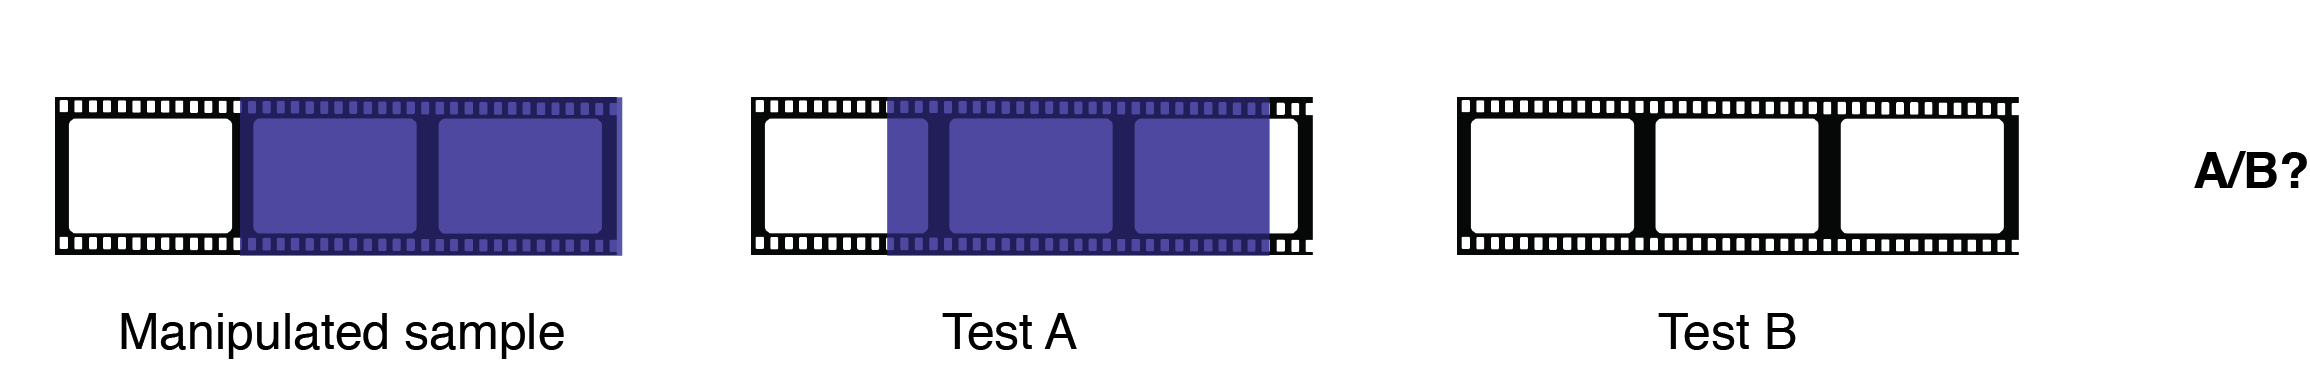
\includegraphics[width=12cm]{img/fire5protocol.png}
                \caption{An altered (filtered or inverted) sample was followed by two untouched tests, one of which contained the sample.}     
        \end{subfigure}
\caption{Experiment 6: design summary and trial structure.}
\end{figure}


\subsection{Results}

\paragraph{Accuracy by manipulation}

The following table shows the mean accuracies for each manipulation, as well as the paired-sample $t$-test $p$-value between that condition and the no-manipulation trials.

\begin{center}
\begin{tabular}{ r | l | l  }
\textbf{Sample manipulation} & \textbf{Mean accuracy} & $p$-value from normal\\
\hline
None&  0.766 & N/A \\
Chromatic& 0.743 & 0.11\\
Reversed&  0.727 & 0.05\\
Inverted&  0.662 & 0.00\\
\end{tabular}
\end{center}

We also note a significant difference between reversion and inversion ($p$=0.03, paired-samples $t$-test). 

All of the conditions gave accuracy greater than chance ($p<$  0.001, single-sample $t$-tests).


\begin{figure}[htp]
\centering

\begin{subfigure}[b]{\textwidth}
\centering
                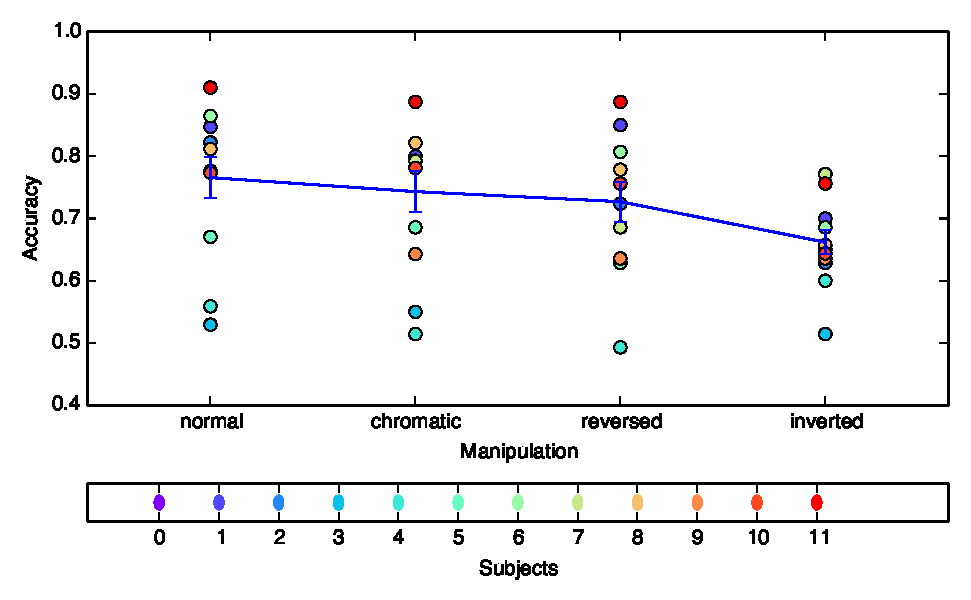
\includegraphics[width=12cm]{img/fig_fire8-manips_correct_manip.pdf}
                \caption{Accuracy against test/sample ratio. Longer tests render the sample harder to find.}
         
        \end{subfigure}
\caption{Experiment 6: effects of each manipulation.}
\end{figure}

\subsection{Discussion}

In terms of design, no-manipulation condition of this experiment exactly replicates the (0.2 second sample, 0.24 second test) condition of experiment 1 (p. \pageref{ex1:accs}). Results were also comparable: accuracy was exactly 0.766 in both cases. As completely different subjects were used, this is useful evidence that we used a large enough sample size.

\paragraph{Colour}
While hue reversal drops the mean by 2 percentage points, a paired-samples $t$-test shows a low probability of difference from the mean ($p$=0.11). Observers do not require the correct colour in order to match fire samples.

\paragraph{Reversal}

Reversing a video clip alters many of its simple motion properties (such as direction of motion) but not certain higher-level motion properties, such as speed. It also does not alter the position of salient motion features: if for example a salient curling flame is tracked in the upper left of the frame, its position will not have changed in the reversed stimulus. Provided that it is just as salient when played in reverse (which small flames usually are, due to their luminance), it will be easily detectable.

Here reversion is associated with a 3.9 percentage point drop in accuracy.

\paragraph{Inversion} 
Inversion alters the local processing of motion features found in fire clips: it transforms upwards motion into downwards motion and leftwards into righwards. It does not, however, alter any of the temporal properties of the clip, either locally or globally.

Inverting a video clip alters the spatial location of all the features contained therein. The signature of a fire clip is not merely a bag of features; each feature is linked to its location in space (``a flare in the the upper left of the frame"). This information is disrupted by inversion.

Here inversion is associated with a 10 percentage point drop in accuracy.

\paragraph{Comparison}

The accuracy drop under inversion (10 p.p.) is much larger than that under reversal (3.9 p.p). For clips of length 0.2 s, then, spatial properties are much more important than temporal properties. Subjects are helped much more by knowing where features are in the image, than when they occur.

Subjects definitely have \textit{some} temporal resolution during the 0.2 second period: persistence of vision blurs details together within a window of 0.04 s\cite{edridge1945persistence}, a much shorter duration than the clips shown here. However, the information derived from the spatial location of features is much more important than temporal information.
